%%%%%%%%%%%%%%%%%%%%%%%%%%%%%%%%%%%%%%%%%
% Beamer Presentation
% LaTeX Template
% Version 1.0 (10/11/12)
%
% This template has been downloaded from:
% http://www.LaTeXTemplates.com
%
% License:
% CC BY-NC-SA 3.0 (http://creativecommons.org/licenses/by-nc-sa/3.0/)
%
%%%%%%%%%%%%%%%%%%%%%%%%%%%%%%%%%%%%%%%%%

%----------------------------------------------------------------------------------------
%	PACKAGES AND THEMES
%----------------------------------------------------------------------------------------

\documentclass{beamer}

\mode<presentation> {

% The Beamer class comes with a number of default slide themes
% which change the colors and layouts of slides. Below this is a list
% of all the themes, uncomment each in turn to see what they look like.

%\usetheme{default}
%\usetheme{AnnArbor}
%\usetheme{Antibes}
%\usetheme{Bergen}
%\usetheme{Berkeley}
%\usetheme{Berlin}
%\usetheme{Boadilla}
%\usetheme{CambridgeUS}
%\usetheme{Copenhagen}
%\usetheme{Darmstadt}
%\usetheme{Dresden}
%\usetheme{Frankfurt}
%\usetheme{Goettingen}
%\usetheme{Hannover}
%\usetheme{Ilmenau}
%\usetheme{JuanLesPins}
%\usetheme{Luebeck}
\usetheme{Madrid}
%\usetheme{Malmoe}
%\usetheme{Marburg}
%\usetheme{Montpellier}
%\usetheme{PaloAlto}
%\usetheme{Pittsburgh}
%\usetheme{Rochester}
%\usetheme{Singapore}
%\usetheme{Szeged}
%\usetheme{Warsaw}

% As well as themes, the Beamer class has a number of color themes
% for any slide theme. Uncomment each of these in turn to see how it
% changes the colors of your current slide theme.

%\usecolortheme{albatross}
%\usecolortheme{beaver}
%\usecolortheme{beetle}
%\usecolortheme{crane}
%\usecolortheme{dolphin}
%\usecolortheme{dove}
%\usecolortheme{fly}
%\usecolortheme{lily}
%\usecolortheme{orchid}
%\usecolortheme{rose}
%\usecolortheme{seagull}
%\usecolortheme{seahorse}
%\usecolortheme{whale}
%\usecolortheme{wolverine}

%\setbeamertemplate{footline} % To remove the footer line in all slides uncomment this line
%\setbeamertemplate{footline}[page number] % To replace the footer line in all slides with a simple slide count uncomment this line

%\setbeamertemplate{navigation symbols}{} % To remove the navigation symbols from the bottom of all slides uncomment this line
}
\usepackage{graphics}
\usepackage{graphicx} % Allows including images
\usepackage{booktabs} % Allows the use of \toprule, \midrule and \bottomrule in tables
\usepackage{algorithmic}
\usepackage{appendixnumberbeamer}
\usepackage{hyperref}

\newcommand{\obar}[1]{\ensuremath{\overline{ #1 }}}
\newcommand{\iid}{\ensuremath{\stackrel{\textrm{iid}}{\sim}}}
\newcommand{\op}[2]{{\ensuremath{\underset{ #2 }{\operatorname{ #1 }}~}}}
\newcommand{\norm}[1]{{ \ensuremath{ \left\lVert  #1 \right\rVert  }  }}
\newcommand{\cov}{ \ensuremath{ \textrm{cov} } }
\newcommand{\var}{ \ensuremath{ \textrm{var} } }
\newcommand{\tr}{ \ensuremath{ \textrm{trace} } }
\newcommand{\df}{ \ensuremath{ \textrm{df} } }
\newcommand{\R}{ \ensuremath{ \mathbb{R} }}


%----------------------------------------------------------------------------------------
%	TITLE PAGE
%----------------------------------------------------------------------------------------

\title[Canned Project]{CSE 380: Final Project} % The short title appears at the bottom of every slide, the full title is only on the title page

\subtitle{Canned Project}

\author{Evan Ott} % Your name

\date{December 9, 2016} % Date, can be changed to a custom date
%\AtBeginSection[]
%{
% \begin{frame}<beamer>
% \frametitle{Plan}
% \tableofcontents[currentsection]
% \end{frame}
%}
\begin{document}

\begin{frame}
\titlepage % Print the title page as the first slide
\end{frame}

\begin{frame}
\frametitle{Overview} % Table of contents slide, comment this block out to remove it
\tableofcontents % Throughout your presentation, if you choose to use \section{} and \subsection{} commands, these will automatically be printed on this slide as an overview of your presentation
\end{frame}

%----------------------------------------------------------------------------------------
%	PRESENTATION SLIDES
%----------------------------------------------------------------------------------------
%------------------------------------------------

\section{Third-Party Libraries}
\begin{frame}
\frametitle{Third-Party Libraries}
\begin{description}
\item[Catch] unit testing, header-defined
\item[Eigen] working with vectors and matrices easily, header-defined
\item[HDF5] output format to store data
\item[GSL] scientific library
\item[INIReader] way to define configuration options easily, header-defined 
\end{description}
\end{frame}


\section{Problem 1}
\begin{frame}
\frametitle{Problem 1}
For this simple problem, I solved the simple ODE
$$\dot{y}(t) = -0.1\cdot y(t)$$
which of course has the solution
$$y(t)=y(t_0) e ^{-0.1(t - t_0)}$$
for an initial condition specified at $t_0$.
\end{frame}

\subsection{Results}
\begin{frame}
\frametitle{Results}
\begin{center}
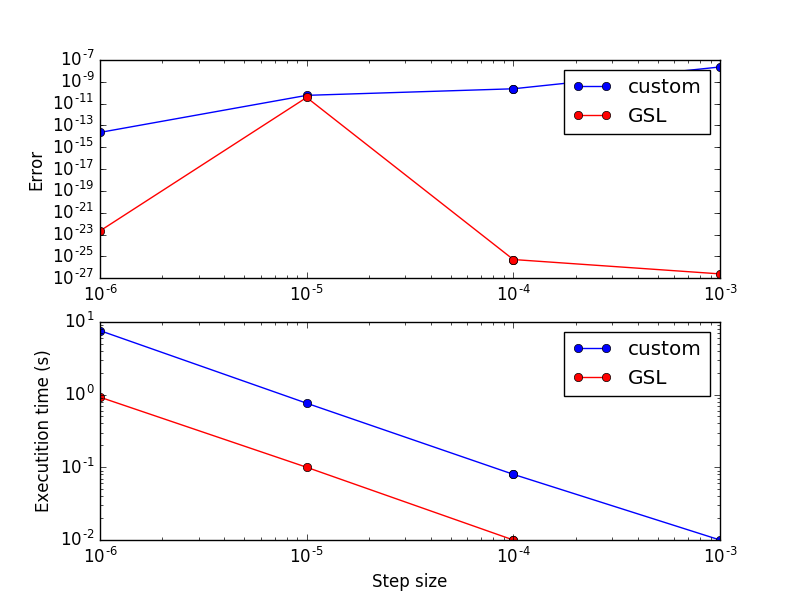
\includegraphics[scale = 0.5]{/Users/Evan/GitProjects/cse380/project/pr1_performance.png}
\end{center}
\end{frame}

\begin{frame}
\frametitle{Results}
\begin{itemize}
\item My implementation of forward Euler is slower than GSL's RK4 method on the same step size
\item My implementation is also less accurate than GSL's RK4 on the same step size \pause
\item This shouldn't be surprising, as forward Euler is in general less accurate than more general Runge-Kutta methods. Furthermore, I decided to use \texttt{Eigen} for handling vectors for problem 2 and the same overhead is present here.
\item Not entirely sure why GSL does relatively poorly for $h=10^{-5}$, but perhaps the larger step sizes were spuriously accurate
\end{itemize}
\end{frame}

\section{Problem 2}
\begin{frame}
\frametitle{Problem 2}
I used \emph{Mathematica} to solve the system of ODEs for the following analytical solutions
\begin{align*}
x(t)&=\frac{20 \tau  e^{-\frac{t}{\tau }} \left(\tau  \omega  \sin (t \omega )+e^{t/\tau }-\cos (t \omega )\right)}{\tau ^2 \omega ^2+1}\\
y(t)&=-\frac{20 \tau  e^{-\frac{t}{\tau }} \left(\tau  \omega  e^{t/\tau }-\tau  \omega  \cos (t \omega )-\sin (t \omega )\right)}{\tau ^2 \omega ^2+1}\\
z(t)&=2 \tau  e^{-\frac{t}{\tau }} \left(e^{t/\tau }-1\right)
\end{align*}
\end{frame}

\subsection{Simulation Results}
\begin{frame}
\frametitle{Simulation Results}
This is a high-resolution result computed on Stampede for 1M iterations with a step size of 0.0001 (RK4).

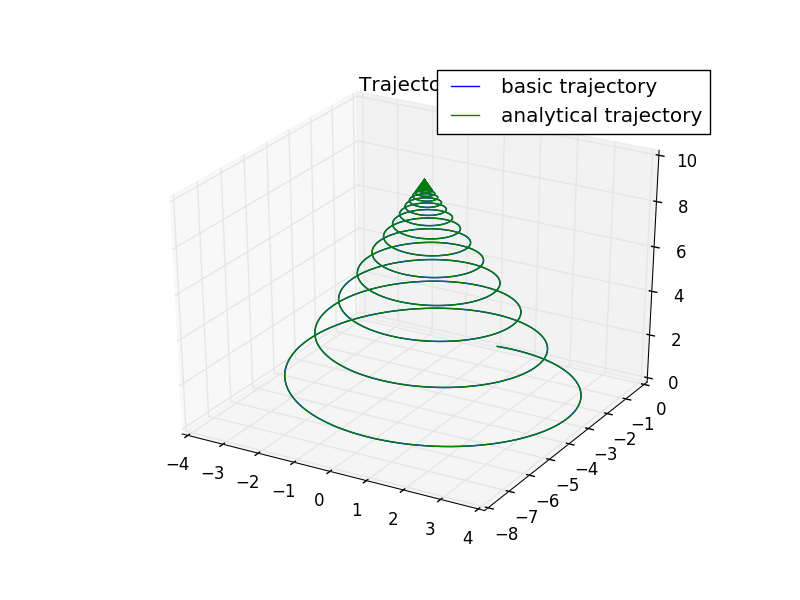
\includegraphics[scale = 0.5]{/Users/Evan/GitProjects/cse380/project/highresTrajectory3d.png}
\end{frame}

\begin{frame}
\frametitle{Simulation Results}
This is a lower-resolution result computed on Stampede for 10K iterations with a step size of 0.01 (RK4).

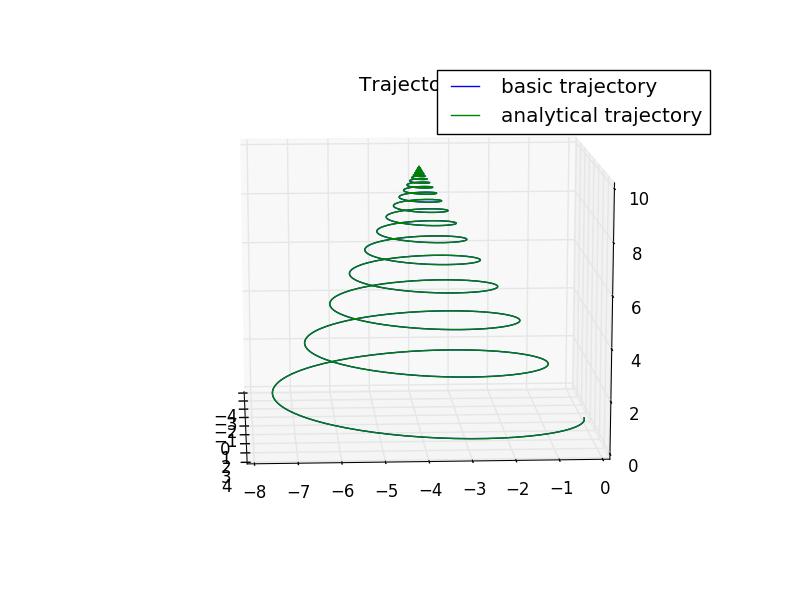
\includegraphics[scale = 0.5]{/Users/Evan/GitProjects/cse380/project/lowresTrajectory3d.png}
\end{frame}

\begin{frame}
\frametitle{Simulation Results}
This is a minimal-resolution result computed on Stampede for 500 iterations with a step size of 0.2 (RK4).

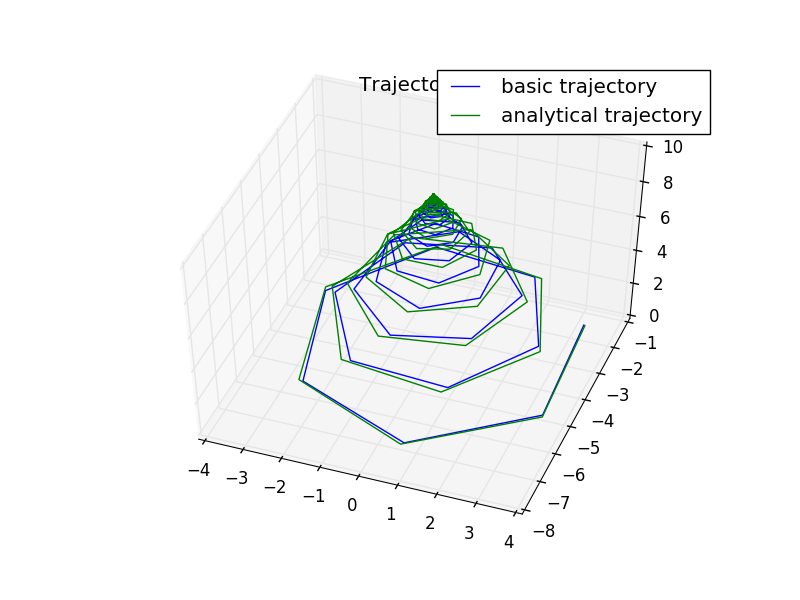
\includegraphics[scale = 0.5]{/Users/Evan/GitProjects/cse380/project/minresTrajectory3d.png}
\end{frame}

\begin{frame}%[allowframebreaks] % will generate multiple pages.
\frametitle{References}
\bibliographystyle{plainnat}
\bibliography{/Users/Evan/GitProjects/tex-docs/references}
\end{frame}


\appendix
\begin{frame}
\frametitle{Appendix A}

\end{frame}


\end{document} 
